% 1959 年全国卷第 8 题：角 B=60°、AC=4 的三角形示意图。
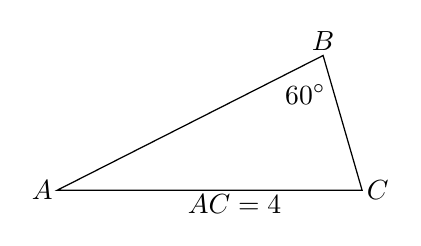
\begin{tikzpicture}[scale=0.9, line width=0.45pt,
  every node/.style={inner sep=1.5pt}]
  \coordinate (A) at (-2.5,0); \coordinate (C) at (1.8,0); \coordinate (B) at (1.25,1.9);
  \draw (A)--(B)--(C)--cycle;
  \node[anchor=east] at (A) {$A$}; \node[anchor=south] at (B) {$B$}; \node[anchor=west] at (C) {$C$};
  \node[anchor=north] at (0,0) {$AC=4$};
  \node at (1.0,1.35) {$60^\circ$};
\end{tikzpicture}
